% !TeX root = verslag.tex
\documentclass{article}
\usepackage[dutch]{babel}
\usepackage{float}
\usepackage{mwe}
\usepackage{hyperref}
\usepackage{csquotes}
\usepackage[table,xcdraw]{xcolor}
\usepackage[sorting=none]{biblatex}
\usepackage[table,xcdraw]{xcolor}
\usepackage{siunitx}
\bibliography{bronnen.bib}
\hypersetup{
  colorlinks=true, % color links instead of border
  linkcolor=blue!50!black,
  urlcolor=blue!50!black
}
\hypersetup{
  colorlinks=true, % color links instead of border
  linkcolor=blue!50!black,
  urlcolor=blue!50!black,
  citecolor=blue!50!black,
  pdftitle={Sensebox_Documents},
  pdfauthor={Joost Visser},
  breaklinks=true
}
\newcommand{\contents} {
  {
    \hypersetup{hidelinks}
    \tableofcontents
  }
  \clearpage
}
% Remove this in your fork if you are cool
\usepackage{lipsum}

% Yea, I got a bunch of custom styling, stored in ./style/ . It's all pretty, self explanatory.
% absolutely incredible document format made by yours truly
% - Jorn Veken, 2022
\usepackage{xcolor}
\usepackage{fontspec}
\usepackage[a4paper, total={6in, 8in}]{geometry}
\usepackage{multicol}

% Background style
\definecolor{page_bg}{rgb}{1.0, 1.0, 1.0}
\pagecolor{page_bg}

% Foreground style
\definecolor{page_fg}{rgb}{0.1, 0.1, 0.1}

\defaultfontfeatures{RawFeature={+axis={wght=100}}}
\setmainfont[
    Path = ./style/fonts/, 
    UprightFont = *-Regular,
    BoldFont = *-Bold,
    ItalicFont = *-Italic,
    ]
{MainFont}

% Default text style
\color{page_fg}
% absolutely incredible document format made by yours truly

% Headers and footer definitions
% Include before document begin

\usepackage{fancyhdr}
\pagestyle{fancy}
\fancyhf{}

% Header
\lhead{Joost Visser}
\rhead{Pagina \thepage}

% Footer
\rfoot{\today}
\lfoot{Lectoraat Smart Driven Data Society \& Inholland Alkmaar}
% absolutely incredible document format made by yours truly
% - Jorn Veken, 2022
% Definitions for code blocks
% Include document begin
\usepackage{listings}
\usepackage{xcolor}
\usepackage{fontspec}
\usepackage[most]{tcolorbox}

% Load code font
\setmonofont[
    Path = ./style/fonts/, 
    UprightFont = *-Regular,
    BoldFont = *-Bold,
    ItalicFont = *-Italic,
    ]
{Codeblock}

% Basic
\definecolor{color_bg}{rgb}{1.0, 1.0, 1.0}
\definecolor{color_fg}{rgb}{0.2, 0.2, 0.2}

% Keywords
\definecolor{color_comment}{rgb}{0.5, 0.3, 1.0}
\definecolor{color_keyword}{rgb}{1.0, 0.3, 0.5}
\definecolor{color_string}{rgb}{0.8, 0.4, 0.4}

% Codeblock specific
\definecolor{color_linenum}{rgb}{0.3, 0.3, 0.3}

% Style definition
\lstdefinestyle{codeblock_default}{
    backgroundcolor = \color{color_bg},   
    commentstyle    = \it\color{color_comment},
    keywordstyle    = \bf\color{color_keyword},
    numberstyle     = \bf\tiny\color{color_linenum},
    stringstyle     = \color{color_string},
    basicstyle      = \small\ttfamily\color{color_fg},
    % Spacing
    breakatwhitespace = false,
    breaklines  = true,                 
    captionpos  = b,                    
    keepspaces  = true,                 
    numbers     = left,                    
    numbersep   = 5pt,                  
    showspaces  = false,        
    % Tabs and Space visibility
    showstringspaces = false,
    showtabs = false,                  
    tabsize  = 2
}

% Set style
\lstset{style=codeblock_default}

\title{\LARGE{Bestellingen document}\\\normalsize{Wat is er besteld?}}
\author{Joost Visser (628941@student.inholland.nl)}
\date{\today}

\begin{document}

    % This is the first page of the document
    % --------------------------------------
    \maketitle
    \vspace{8em}
    \begin{figure}[H]
        \centering
        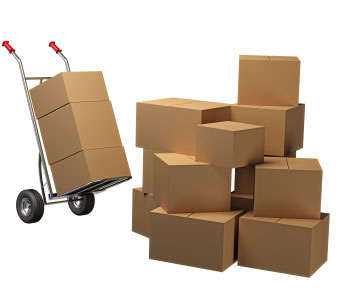
\includegraphics[width=30em]{fotos/cover.jpg}
        \caption[]{Bestellingen}
    \end{figure}
    \vfill
    \newpage
    % --------------------------------------

    % Inhoudsopgave
    \tableofcontents
    \newpage

    % To use codeblocks, write \begin{codeblock}{} \end{codeblock}
    % absolutely incredible document format made by yours truly
% - Jorn Veken, 2022
\newtcblisting{codeblock}[2][]{%
    enhanced, title=#2, 
    colback=white,
    attach boxed title to top left = {xshift=5mm,yshift=-2mm},
    fonttitle=\ttfamily, coltitle=white,
    listing only,listing options={language=C, basicstyle=\ttfamily\footnotesize},#1}

% Here's a code snippet for code blocks.
\iffalse
begin{codeblock}{main.py}
   import cv2 as cv
   
   def main()
       print('Hello, world!')
       return
   
   if __name__ == '__main__' :
       main()
\end{codeblock}
\fi

    % Here all the sections go. Stored in ./sections/
    % --------------------------------------
    \begin{flushleft}

    \section{Sensoren}
    \label{sec:Sensoren}
    % leg hier de afwegingen die gedaan zijn uit over welke sensor gekozen is en waarom die.
% bijvoorbeeld hij was leverbaar en viel binnen de meet-range en precisie die is verteld in de eigenschappen section of requirements
In deze sectie wordt de verantwoording voor de verschillende gekozen sensoren uitgelicht. Als requirement moesten alle sensoren bestelbaar zijn via \href{https://nl.farnell.com}{Farnell}, \href{https://nl.mouser.com}{Mouser}, \href{https://nl.rs-components.com}{rs-components} of \href{https://kiwi-electronics.nl}{Kiwi-electronics}. Verder is het gewenst dat de sensor via I2C of analoog werkt en dat de sensor werkt op 3v3. 

\subsection{MIX8410 - Zuurstof}
\label{sec:mix}
De MIX8410 is gekozen als O$_2$ sensor omdat deze een nauwkeurigheid heeft van 0.1\% een meetbereik heeft van 0 tot 25\% en een response time van minder dan 10 seconden. Verder is dit de enige sensor die op dit moment op de aangegeven sites bestelbaar is. 

\subsection{AS7262 - licht spectrum}
\label{sec:as}
De AS7262 is gekozen als licht spectrum sensor. De sensor heeft 6 verschillende kanalen op verschillende golflengtes, tussen de 450nm en 650nm die allemaal een eigen kleur representeren, met een nauwkeurigheid van $\pm$12\%. De AS7262 kan worden aangesloten via I2C of UART en werkt op 3v3. Er is gekozen voor deze oplossing omdat uit de 5 verschillende golflengtes het soort kamer licht kan worden bepaald. 

\subsection{Sensirion SCD30 - CO2, Hum, Temp}
\label{sec:SCD30}

De Sensirion SCD30 is een pcb met verschillende sensoren. Deze is gekozen voor zijn CO$_2$ sensor. Hiernaast beschikt de sensor over een luchtvochtigheid en temperatuur sensor. De CO$_2$ sensor heeft een meetbereik van 400-10000ppm met een nauwkeurigheid van $\pm$30ppm en kan een meeting doen elke 2 seconden. De luchtvochtigheid sensor kan tussen de 0\% en 100\%RH (Relative Humidity) meten met een nauwkeurigheid van $\pm$3\% en kan een meeting doen elke 8 seconden. De temperatuur sensor kan tussen de -40 en 70 graden C° met een nauwkeurigheid van $\pm$0.4 C° en kan een meeting doen elke 10 seconden. Doordat de sensor 3 verschillende attributen meet die allemaal binnen de gestelde meetbereik en nauwkeurigheid valt en eveneens ook bestelbaar is via één van de 4 beschikbare sites is deze sensor gekozen.\\

De Sensirion SCD30's data wordt verder samen verwerkt met de Ambimate Sensor module's Temperatuur, en luchtvochtigheid's sensor gezien deze twee een vergelijkbare nauwkeurigheid hebben.

\subsection{MAX4466 - Geluid}
\label{sec:max}
De MAX4466 sensor is gekozen als geluid sensor. Deze sensor is gekozen omdat op de sensor een ingebouwde versterkingsregelaar zit voor het versterken van het binnenkomend signaal. Verder is het signaal analoog dus kan de sensor continu worden uitgelezen. De sensor werkt op 3v3 waardoor geen interne conversie nodig is op het PCB. De microfoon kan tussen de 20 en 20000Hz ontvangen met een gevoeligheid van -44 $\pm$ 2dB. De frequentie kan verder worden omgezet naar dB via online beschikbare libraries. Hierdoor is het mogelijk om niet alleen de luidheid maar ook de toonhoogte te bepalen.

\subsection{CCS811 - VOC, eCO2}
\label{sec:mate}
De CCS811 is een VOC sensor die gebruik maakt van I2C met een supply voltage van 3v3. Hiernaast heeft deze sensor ook een temperatuur en humidity nodig. De SCD30 beschikt hierover en  is hierom ook nodig om uit te kunnen lezen. De VOC sensor heeft een meetbereik tussen de 0-1187ppb. De eCO$_2$ wordt bepaald op basis van de VOC en heeft een meetbereik van 400-8192ppm. Vanwege de veel verschillende attributen die deze module kan meten en ook binnen de gestelde meetbereik en nauwkeurigheid valt, eveneens als beschikbaar via één van de 4 beschikbare sites is deze sensor gekozen. Deze sensor is ook gekozen omdat het kan worden gebruikt met de andere sensoren en deze sensor gebruikt ook I2C wat het aansluiten makkelijker maakt.\\

\subsection{TSL2591 - licht intensiteit}
\label{sec:TSL}
De TSL2591 is gekozen als licht intensiteit sensor. De sensor kan tussen de 188\si{\micro Lux} en 88000\si{Lux}. Eveneens kan de TSL2591 ook infrarood en full-spectrum of human-visible light meten. De keuze voor de sensor is vanwege zijn grote meetbereik en het communicatie protocol; I2C op 3v3. Deze sensor is net zoals de andere ook beschikbaar op één van de aangegeven sites.

\subsection{PMSA003I - fijnstof}
\label{sec:smuart}
De PMSA003I Laser Dust sensor is gekozen als fijnstof sensor. De sensor communiceert via I2C en heeft een 3v3 supply voltage nodig. Deze sensor is gekozen omdat deze beschikbaar is met een betaalbare prijs en gebruik maakt van I2C. De sensor kan tussen de 0.3\si{\micro\meter} en 10\si{\micro\meter} deeltjes meten. Verder heeft de sensor een meetbereik tussen de 1 en 999\si{\micro\gram\per\cubic\meter} en een nauwkeurigheid van 1\si{\micro\gram\per\cubic\meter}. De sensor heeft 5 seconden nodig om op te starten en kan daarna elke seconden worden uitgelezen.



      
     \section{Bestellingen}
     \label{sec:Bestellingen}
     \begin{table}[H]
\centering
\begin{tabular}{lllll}
\hline
\multicolumn{1}{|l|}{SensorID} & \multicolumn{1}{l|}{Sensornaam}       & \multicolumn{1}{l|}{Meet}                & \multicolumn{1}{l|}{Prijs (in euro, incl. BTW)} & \multicolumn{1}{l|}{Bestellink}                                                                                                                       \\ \hline
\multicolumn{1}{|l|}{1}        & \multicolumn{1}{l|}{MIX8410}          & \multicolumn{1}{l|}{O2}                  & \multicolumn{1}{l|}{35,13}                      & \multicolumn{1}{l|}{\href{https://nl.mouser.com/ProductDetail/Seeed-Studio/101990680?qs=DPoM0jnrROWBX\%2FfANB1IYw\%3D\%3D}{Link}}                     \\ \hline
\multicolumn{1}{|l|}{2}        & \multicolumn{1}{l|}{SCD30}            & \multicolumn{1}{l|}{CO2,   Hum, Temp}    & \multicolumn{1}{l|}{55,64}                      & \multicolumn{1}{l|}{\href{https://nl.rs-online.com/web/p/temperature-humidity-sensor-ics/1720552/}{Link}}                                             \\ \hline
\multicolumn{1}{|l|}{3}        & \multicolumn{1}{l|}{MQ-7}             & \multicolumn{1}{l|}{CO}                  & \multicolumn{1}{l|}{6,14}                       & \multicolumn{1}{l|}{\href{https://nl.mouser.com/ProductDetail/474-SEN-09403}{Link}}                                                                   \\ \hline
\multicolumn{1}{|l|}{4}        & \multicolumn{1}{l|}{TSL2591}          & \multicolumn{1}{l|}{Licht   intensiteit} & \multicolumn{1}{l|}{5,89}                       & \multicolumn{1}{l|}{\href{https://nl.mouser.com/ProductDetail/Adafruit/1980?qs=sGAEpiMZZMsKEdP9slC0YSnuTSFmm1LYraEQV\%252B1EsJM\%3D}{Link}}           \\ \hline
\multicolumn{1}{|l|}{5}        & \multicolumn{1}{l|}{AS7262}           & \multicolumn{1}{l|}{Licht   spectrum}    & \multicolumn{1}{l|}{16,9}                       & \multicolumn{1}{l|}{\href{https://nl.mouser.com/ProductDetail/Adafruit/3779?qs=\%2Fha2pyFaduhIK8PZSZbRzZsXMtLLCRlN2lsYwgiwgTg\%}{Link}}               \\ \hline
\multicolumn{1}{|l|}{6}        & \multicolumn{1}{l|}{CCS811}           & \multicolumn{1}{l|}{VOC}                 & \multicolumn{1}{l|}{23,95}                      & \multicolumn{1}{l|}{\href{https://www.kiwi-electronics.com/nl/adafruit-ccs811-air-quality-sensor-breakout-voc-eco2-3205?search=CCS811}{Link}}         \\ \hline
\multicolumn{1}{|l|}{7}        & \multicolumn{1}{l|}{MAX4466}          & \multicolumn{1}{l|}{Geluid}              & \multicolumn{1}{l|}{8,25}                       & \multicolumn{1}{l|}{\href{https://nl.farnell.com/adafruit/1063/silicon-manufacturer-maxim-integrated/dp/2419156?st=MAX4466}{Link}}                    \\ \hline
\multicolumn{1}{|l|}{8}        & \multicolumn{1}{l|}{PMSA003I}         & \multicolumn{1}{l|}{Fijnstof}            & \multicolumn{1}{l|}{52,95}                      & \multicolumn{1}{l|}{\href{https://www.kiwi-electronics.com/nl/adafruit-pmsa003i-air-quality-breakout-stemma-qt-qwiic-10427?search=PMSA003I\%20}{Link}} \\ \hline
\end{tabular}
\caption{Bestellijst sensoren}
\label{tab:bestellijst}
\end{table}

De sensoren beschikken over de volgende elektrische eigenschappen
\begin{table}[H]
    \centering
    \begin{tabular}{|l|l|l|l|l|l|l|}
    \hline
        Naam & Protocol & Supply & Logic & Meet & Datasheet & shop  \\ \hline    
        MIX8410 & analoog & 3-5v & 3v3  & O$_2$ & \href{https://nl.mouser.com/datasheet/2/744/MIX8410_Electrochemical_Oxygen_Gas_Sensor_V1_6-1903280.pdf}{Link} & \href{https://nl.mouser.com/ProductDetail/Seeed-Studio/101990680?qs=DPoM0jnrROWBX\%2FfANB1IYw\%3D\%3D}{Link} \\ \hline
        Sensirion SCD30 & I2C, UART & 0.3V - 6.0V & 3.3v - 5.5v  & CO2, Hum, Temp & \href{https://docs.rs-online.com/2d49/0900766b816b6f9d.pdf}{Link} & \href{https://nl.rs-online.com/web/p/temperature-humidity-sensor-ics/1720552/}{Link} \\ \hline
        TSL2591 & I2C & 3v3 & 3v3  & licht intensiteit & \href{https://nl.mouser.com/datasheet/2/737/TSL25911_Datasheet_EN_v1-2490266.pdf}{Link} & \href{https://nl.mouser.com/ProductDetail/Adafruit/1980?qs=sGAEpiMZZMsKEdP9slC0YSnuTSFmm1LYraEQV\%252B1EsJM\%3D}{Link} \\ \hline
        AS7262 & I2C, UART & 3-5v & 3v3  & Light spectrum & \href{https://learn.adafruit.com/adafruit-as7262-6-channel-visible-light-sensor/overview}{Link} & \href{https://www.kiwi-electronics.nl/nl/adafruit-as7262-6-channel-visible-light-color-sensor-3575}{Link} \\ \hline
        CS811 & I2C & 3v3 & 3v3  & VOC & \href{https://learn.adafruit.com/adafruit-ccs811-air-quality-sensor}{Link} & \href{https://www.kiwi-electronics.com/nl/adafruit-ccs811-air-quality-sensor-breakout-voc-eco2-3205?search=CCS811}{Link} \\ \hline
        MAX4466 & analog & 2.4-5.5v & 2.4-5.5V  & geluid & \href{https://datasheets.maximintegrated.com/en/ds/MAX4465-MAX4469.pdf}{Link} & \href{https://www.kiwi-electronics.nl/nl/elektretmicrofoon-versterker-max4466-met-instelbare-gain-806}{Link} \\ \hline
        PMSA003I & I2C & 5v & 3v3  & Fijnstof & \href{hhttps://learn.adafruit.com/pmsa003i}{Link} & \href{https://www.kiwi-electronics.com/nl/adafruit-pmsa003i-air-quality-breakout-stemma-qt-qwiic-10427}{Link} \\ \hline
    \end{tabular}
    \caption{Elektrische eigenschappen van de sensoren}
    \label{tab:eingeschappensensoren}
\end{table}

\newpage
De sensoren beschikken over de volgende meet-limieten.
\begin{table}[H]
\centering
\begin{tabular}{|l|l|l|l|l|l|}
\hline
SensorID & Meet              & Meetbereik        & Nauwkeurigheid & Herhaalbaarheid & Reactietijd       \\ \hline
1        & O2                & 0-25\%            & 0.1            & ±2\%            & \textless{}10s    \\ \hline
2        & CO2               & 0-40000ppm        & ±30ppm         & ±10ppm          & 20s               \\ \hline
2        & Luchtvochtigheid  & 0\%RH - 100\%RH   & ±3\%RH         & ±0.1\%RH        & 8s                \\ \hline
2        & Temperatuur       & -40-70°C          & ±0.4°C         & ±0.14°C         & \textgreater{}10s \\ \hline
4        & Licht intensiteit & up to 88,000 uLux & 188 uLux       & -               & -                 \\ \hline
5        & Licht spectrum    & 450-650nm         & -              & -               & -                 \\ \hline
6        & Temp              & 5-50°C            & 1°C            & -               & 1s                \\ \hline
6        & Luchtvochtigheid  & 5-95\%RH          & 3\%RH          & -               & 1s                \\ \hline
6        & Lichtintensiteit  & 0-1024 lux        & -              & -               & 1s                \\ \hline
6        & VOC               & 0-1187 ppb        & -              & -               & 60s               \\ \hline
6        & eCO2              & 400-8192ppm       & -              & -               & 60s               \\ \hline
6        & Microfoon         & -                 & -              & -               & \textless{}0.5s   \\ \hline
6        & Beweging          & -                 & -              & -               & -                 \\ \hline
7        & Geluid            & 200kHz            & -              & -               & -                 \\ \hline
8        & Fijnstof          & PM2.5 output      & -              & -               & -                 \\ \hline
\end{tabular}
\caption{Meetbare eigenschappen, limieten en precisie}
\label{tab:eigenschappen}
\end{table}

%    \end{flushleft}
    % --------------------------------------
    % Sources at the end
    \printbibliography

    \iffalse
    \section{geheime bedreiging}
    Oja, nog even wat.
    
    \vspace{1em}
    Als ik iemand ook maar 1 keer enter zie gebruiken, in plaats van gewoon inz een lange regel door schrijven. Dan wordt ik big sad, wen er aan. Zet word wrap aan. Idc. Wordt een goede latex gebruiker, enter heeft ook een functie namelijk
    \fi

\end{document}